\begin{frame}[t, c]{}{}
  \begin{minipage}{.48\textwidth}
    \centering
    \begin{tikzpicture}
      \node[state] (s1) {\( \bm{s}_1 \)};
      \node[state, below right of=s1] (s2) {\( \bm{s}_2 \)};
      \node[state, below left of=s1] (s4) {\( \bm{s}_4 \)};
      \node[state, below left of=s2] (s3) {\( \bm{s}_3 \)};
      
      \draw (s1) edge[loop above] node {\(l_{11}\)} (s1);
      \draw (s1) edge[bend left] node {\(l_{21}\)}  (s2);
      
      \draw (s2) edge[loop right]  node {\(l_{22}\)} (s2);
      \draw (s2) edge[bend left]  node {\(l_{32}\)} (s3);
      
      \draw (s3) edge[bend left]  node {\(l_{43}\)} (s4);
      \draw (s3) edge[loop below]  node {\(l_{33}\)} (s3);
      
      \draw (s4) edge[bend left]  node {\(l_{14}\)} (s1);
      \draw (s4) edge[loop left]  node {\(l_{44}\)} (s4);
      
    \end{tikzpicture}
  \end{minipage}%
  \hfill
  \begin{minipage}{.48\textwidth}
    \centering
    {
      \Large\textbf{Appendix}
    }
    
    \bigskip
    
    \rule{\textwidth}{0.001\textwidth}
    
    \bigskip
    
    {
      \large
      \textbf{Miscellaneous}
    }
    
    \medskip
    
    \begin{itemize}
    \item Dynamic Mode Decomposition:
      \begin{itemize}
      \item[\(	\hookrightarrow \)] Theorem \& Proof
      \item[\(	\hookrightarrow	\)] PCA vs.\ CCA vs.\ DMD
      \end{itemize}
      
      \medskip
      
    \item Probabilistic model:
      \begin{itemize}
      \item[\(	\hookrightarrow	\)] How to choose the number of clusters ?
      %\item[\(	\hookrightarrow \)] Maximum Likelihood Estimation of the transition matrix.
      \end{itemize}

      \medskip
      
    \item SINDy with constraints:
      \begin{itemize}
      %\item[\(	\hookrightarrow	\)] Numerical algorithm.
      \item[\(	\hookrightarrow \)] Covariance matrix of the parameters.
      \end{itemize}
      
    \end{itemize}
    
  \end{minipage}
\end{frame}

\begin{frame}[t, c]{Dynamic Mode Decomposition}{Theorem \& Proof}
  \begin{block}{\textbf{Theorem :} Optimal solution to the DMD problem}
  \end{block}

  \medskip
  
  The solution to the DMD problem
  % 
  $$
  \begin{aligned}
    \minimize_{\bm{P}, \bm{Q}} & \| \bm{Y} - \bm{PQ}^H \bm{X} \|_F^2 \\
    \subjecto & \text{rank } \bm{P} = \text{rank } \bm{Q} = r \\
    & \bm{P}^H \bm{P} = \bm{I}
  \end{aligned}
  $$
  % 
  is given by the first $r$ eigenvectors of the symmetric positive definite matrix $\bm{C}_{\bm{yx}} \bm{C}_{\bm{xx}}^{-1} \bm{C}_{\bm{xy}}$.

  \vspace{1cm}
\end{frame}

\begin{frame}[t, c]{Dynamic Mode Decomposition}{Thereom \& Proof}
  \begin{block}{\textbf{Proof :} Haven't had time to write it properly in beamer !}
  \end{block}

  \medskip

  
\end{frame}

\begin{frame}[t, c]{Dynamic Mode Decomposition}{PCA vs.\ CCA vs.\ DMD}
  \begin{block}{\centering \textbf{Principal Component Analysis}}
    $$
    \begin{bmatrix}
      \bm{I} & \bm{0} \\
      \bm{0} & \bm{I}
    \end{bmatrix}
    \begin{bmatrix}
      \bm{P} \\
      \bm{Q}
    \end{bmatrix}
    \boldsymbol{\Uplambda}
    =
    \begin{bmatrix}
      \bm{C}_{\bm{yy}} & \bm{0} \\
      \bm{0} & \bm{C}_{\bm{xx}}
    \end{bmatrix}
    \begin{bmatrix}
      \bm{P} \\
      \bm{Q}
    \end{bmatrix}    
    $$
  \end{block}

  \medskip

  \begin{block}{\centering \textbf{Canonical Correlation Analysis}}
    $$
    \begin{bmatrix}
      \bm{C}_{\bm{yy}} & \bm{0} \\
      \bm{0} & \bm{C}_{\bm{xx}}
    \end{bmatrix}
    \begin{bmatrix}
      \bm{P} \\
      \bm{Q}
    \end{bmatrix}
    \boldsymbol{\Uplambda}
    =
    \begin{bmatrix}
      \bm{0} & \bm{C}_{\bm{yx}} \\
      \bm{C}_{\bm{xy}} & \bm{0}
    \end{bmatrix}
    \begin{bmatrix}
      \bm{P} \\
      \bm{Q}
    \end{bmatrix}    
    $$
  \end{block}

  \medskip

  \begin{block}{\centering \textbf{Dynamic Mode Decomposition}}
    $$
    \begin{bmatrix}
      \bm{I} & \bm{0} \\
      \bm{0} & \bm{0}
    \end{bmatrix}
    \begin{bmatrix}
      \bm{P} \\
      \bm{Q}
    \end{bmatrix}
    \boldsymbol{\Uplambda}
    =
    \begin{bmatrix}
      \bm{0} & \bm{C}_{\bm{yx}} \\
      \bm{C}_{\bm{xy}} & -\bm{C}_{\bm{xx}}
    \end{bmatrix}
    \begin{bmatrix}
      \bm{P} \\
      \bm{Q}
    \end{bmatrix}    
    $$
  \end{block}

  \vspace{1cm}
\end{frame}

%%%%%
%%%%%
%%%%%
%%%%%
%%%%%

\begin{frame}[t, c]{Probabilistic model}{How to choose the number of clusters ?}
  \begin{minipage}{.68\textwidth}
    \begin{itemize}
    \item Various heuristics exist to assess how good our clustering is.
      
      \medskip
      
    \item Calinski \& Harabasz Index : choose the number of clusters based on the ratio of within-cluster and between-cluster dispersions
      % 
      $$
      CH(k) = \frac{tr(\bm{B}_k)}{tr(\bm{W}_k)} \times \frac{n_E -k}{k-1}
      $$
      % 
      where $tr(\bm{B}_k)$ is the between-cluster dispersion and $tr(\bm{W}_k)$ is the within-cluster dispersion.
      
      \medskip
      
    \item Other possible metrics : Silouhette coefficient, Davies-Bouldin Index, etc.
    \end{itemize}
  \end{minipage}%
  \hfill
  \begin{minipage}{.28\textwidth}
    \centering
    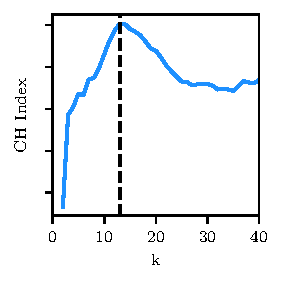
\includegraphics[width=\textwidth]{CH_index}
  \end{minipage}

  \vspace{1cm}
\end{frame}

% \begin{frame}[t, c]{Probabilistic model}{Maximum Likelihood Estimation of the transition matrix}
%   \begin{minipage}{.58\textwidth}
%   \end{minipage}%
%   \hfill
%   \begin{minipage}{.38\textwidth}
%     \centering
%     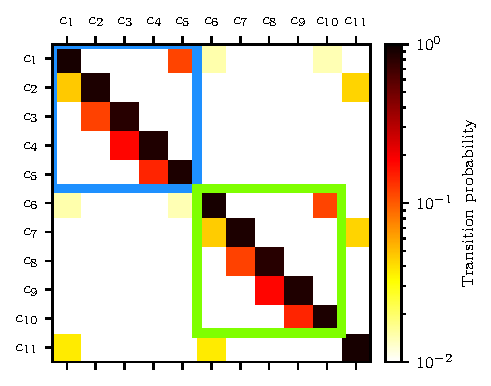
\includegraphics[width=\textwidth]{CROM_transition_matrix}
%   \end{minipage}

%   \vspace{1cm}
% \end{frame}

%%%%%
%%%%%
%%%%%
%%%%%
%%%%%

% \begin{frame}[t, c]{Sparse Identification of Nonlinear Dynamics}{Numerical Algorithm}
% \end{frame}

\begin{frame}[t, c]{Sparse Identification of Nonlinear Dynamics}{Covariance matrix of the parameters}
  \begin{minipage}{.48\textwidth}
    \centering
    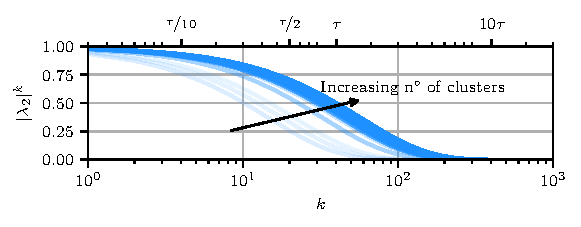
\includegraphics[width=\textwidth]{convergence_crom}
  \end{minipage}%
  \hfill
  \begin{minipage}{.48\textwidth}
    \begin{itemize}
    \item Dynamics of the system are correlated only on a time-scale $\mathcal{O}(\tau)$.
    \item Dataset can be partionned into $n$ independant realizations.
    \end{itemize}
  \end{minipage}

  \bigskip
  
  \begin{minipage}{.48\textwidth}
    \begin{itemize}
    \item One can use \underline{bootstrapping} to estimate the covariance matrix of the parameters.
    \item It then enables us to perform uncertainty quantification when forecasting.
    \end{itemize}
  \end{minipage}%
  \hfill
  \begin{minipage}{.48\textwidth}
  \end{minipage}

  \vspace{1cm}
\end{frame}